%%%%%%%%%%%%%%%%%%%%%%%%%%%%%%%%%%%%%%%%%%%%%%%%%%%%%%%%%%%%%%%%%%%
%%% Documento LaTeX 																						%%%
%%%%%%%%%%%%%%%%%%%%%%%%%%%%%%%%%%%%%%%%%%%%%%%%%%%%%%%%%%%%%%%%%%%
% Título:		Capítulo 5
% Autor:  	Ignacio Moreno Doblas
% Fecha:  	2014-02-01, actualizado 2019-11-11
% Versión:	0.5.0
%%%%%%%%%%%%%%%%%%%%%%%%%%%%%%%%%%%%%%%%%%%%%%%%%%%%%%%%%%%%%%%%%%%
% !TEX root = A0.MiTFG.tex

\chapterbegin{Pruebas}
\label{chp:App3}
\minitoc
En este capítulo se van a presentar diferentes pruebas para comprobar el 
correcto funcionamiento
de cada esquema de codificación, con cada sistema de decisión, una vez han sido 
integrados en el sistema completo de comunicación. 

Para ello se dispone del enlace de luz comentado en el capítulo 3 y que se muestra 
a continuación en la figura \ref{enlace2}

\begin{figure}[ht]
    \centering
    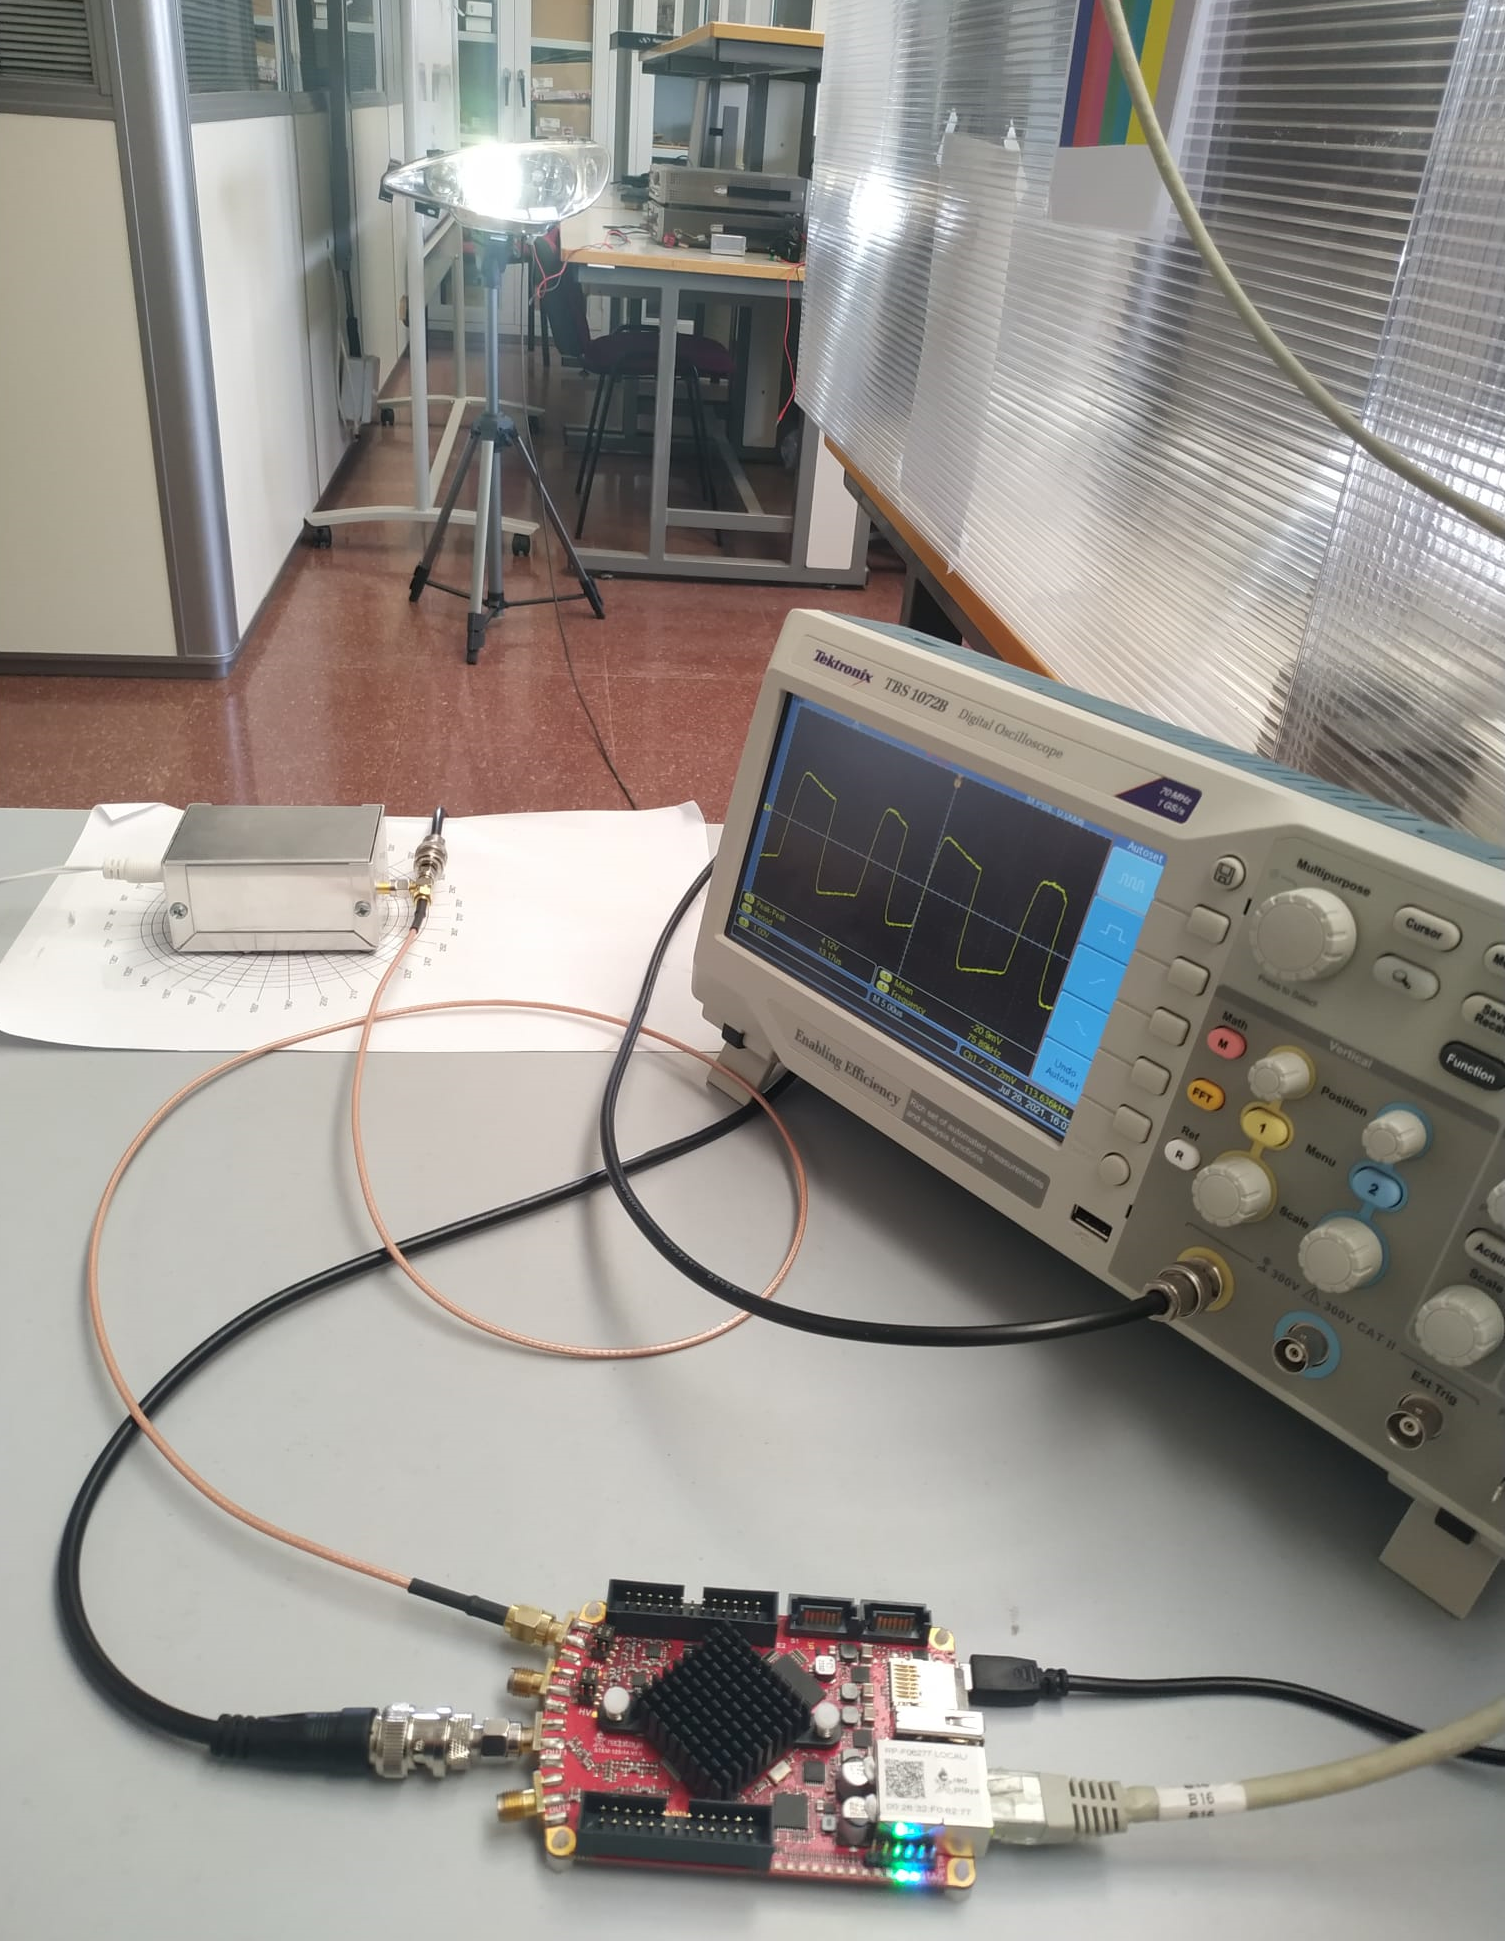
\includegraphics[scale=0.1]{./figuras/Enlace.png}
    \caption{\small{Sistema de transmisión-recepción completo.}}
    \label{enlace2}%
\end{figure}

En la figura \ref{global}, se puede ver la configuración global del sistema para la 
ejecución de esta prueba. 

\begin{figure}[ht]
    \centering
    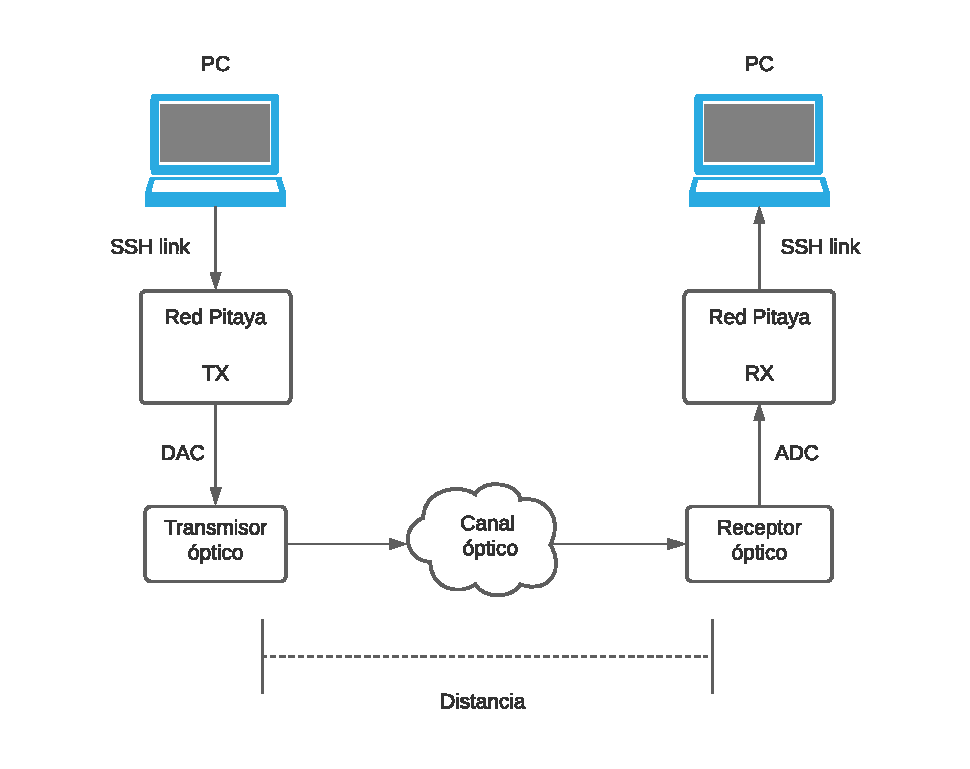
\includegraphics[scale=0.73]{./figuras/sistema_global.pdf}
    \caption{\small{Sistema global para la transmisión-recepción.}}
    \label{global}%
\end{figure}

Para realizar dichas pruebas se van a transmitir 1000 paquetes en los que, cada uno, 
contiene una trama de datos pseudoaleatoria a diferentes distancias ya que es la 
forma de disminuir la amplitud de la señal y por consecuencia, disminuir la 
relación señal a ruido (SNR).

El objetivo de la prueba es comprobar cuántos paquetes llegan correctos y en caso 
contrario de cuántos bits es el error a diferentes distancias y velocidades de 
transmisión para conocer las capacidades de cada esquema de codificación.

Tal y como se observa en la figura anterior, el terminal de una sesión SSH, desde un PC 
remoto conectado a la misma red local que la Red Pitaya, será el encargado de 
controlar el ARM de la placa para ejecutar el programa en lenguaje
C que se ha desarrollado para realizar la transmisión o recepción de los paquetes. 
En las figuras \ref{ok} y \ref{fail} se muestra cómo se reciben los diez primeros 
paquetes. En el terminal se van imprimiendo mensajes en función de
si el paquete se ha recibido correctamente 'Recibido OK', se ha recibido con errores 
en la trama 'Recibido ERROR' o se ha perdido 'Perdido'. Para el caso de que se reciba 
el paquete se muestra en la terminal los 10 primeros bytes de la trama de datos. 

\begin{figure}[ht]
	\centering
	  \begin{minipage}{7cm}
		\centering
		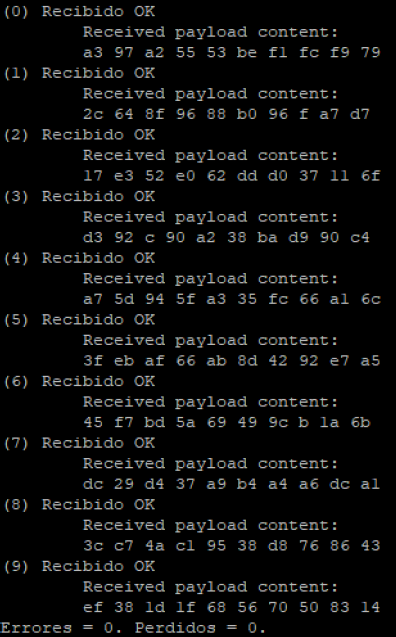
\includegraphics[scale=0.60]{./figuras/putty_rec.png}
		\caption{\small{Recepción correcta de paquetes.}}
		\label{ok}
	  \end{minipage}%
	  \hspace{5mm}
	  \begin{minipage}{7cm}
		\centering
		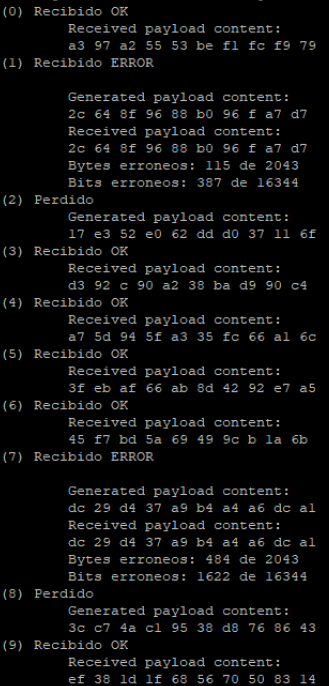
\includegraphics[scale=0.56]{./figuras/putty_rec_fail.png}
		\caption{\small{Recepción errónea de paquetes.}}
		\label{fail}
	  \end{minipage}
\end{figure}

La figura \ref{real} representa una recepción real de una prueba realizada para una 
transmisión
de 1000 paquetes. Se observa como se detalla toda la información correspondiente a la
recepción del paquete siendo la más esencial los paquetes correctos y la BER (tasa de 
error de bit).

\begin{figure}[ht]
    \centering
    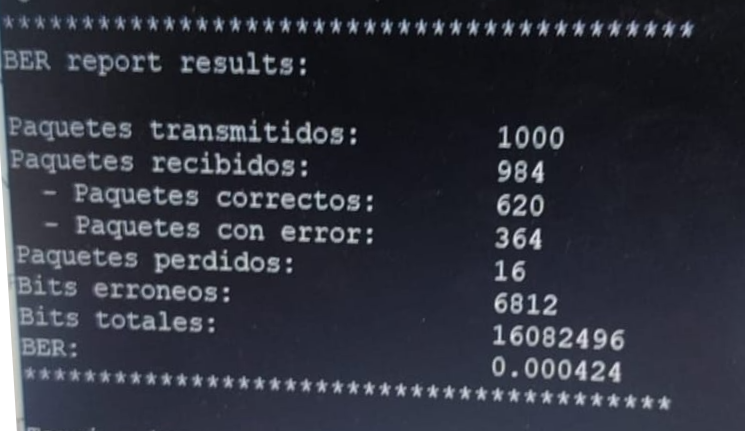
\includegraphics[scale=0.50]{./figuras/1.png}
    \caption{\small{Terminal de recepción.}}
    \label{real}%
\end{figure}

Las pruebas realizadas se van a dividir en diferentes apartados según la distancia 
a la que se han realizado. Cada uno de los apartados muestra 
una tabla con los resultados obtenidos para cada esquema de codificación con su mejor
sistema de decisión, es decir, pulsos alternos con Viterbi,
cancelación de pulsos con Viterbi y 4PPM con \textit{soft-decoding}.

\section{24 metros}

\begin{table}[ht]
	\begin{tabular}{c|c|c|c|}
	\cline{2-4}
														 & \textbf{Paquetes recibidos} & \textbf{Paquetes correctos} & \textbf{BER} \\ \hline
	\multicolumn{1}{|c|}{\textbf{Pulsos Alternos}}       & 1000                        & 1000                        & 0            \\ \hline
	\multicolumn{1}{|c|}{\textbf{Cancelación pulsos}} 	 & 1000                        & 1000                        & 0            \\ \hline
	\multicolumn{1}{|c|}{\textbf{4PPM}}                  & 1000                        & 1000                        & 0            \\ \hline
	\end{tabular}
	\caption{\small{Prestaciones a 24 metros.}}
	\end{table}

\section{40 metros}

Para esta distancia las prestaciones siguen siendo casi perfectas aunque ya 
empieza a notarse un poco la diferencia entre cada esquema de codificación.

\begin{table}[ht]
	\begin{tabular}{c|c|c|c|}
	\cline{2-4}
																				 & \textbf{Paquetes recibidos} & \textbf{Paquetes correctos} & \textbf{BER} \\ \hline
	\multicolumn{1}{|c|}{\cellcolor[HTML]{FFFFFF}\textbf{Pulsos Alternos}}       & 936                         & 912                         & 0.001727     \\ \hline
	\multicolumn{1}{|c|}{\cellcolor[HTML]{FFFFFF}\textbf{Cancelación pulsos}} 	 & 958                         & 958                         & 0            \\ \hline
	\multicolumn{1}{|c|}{\cellcolor[HTML]{FFFFFF}\textbf{4PPM}}                  & 993                         & 993                         & 0            \\ \hline
	\end{tabular}
	\caption{\small{Prestaciones a 40 metros.}}
	\end{table}

\section{54 metros}

A partir de esta distancia las prestaciones de pulsos alternos y de cancelación de 
pulsos son nulas ya que no se recibe ningún paquete. Para ambos casos la culpa es de 
la cabecera porque al hacer el cálculo del CRC desecha el paquete. 
Sin embargo, las prestaciones de 4PPM siguen siendo excelentes.

\begin{table}[ht]
	\begin{tabular}{c|c|c|c|}
	\cline{2-4}
														 & \textbf{Paquetes recibidos} & \textbf{Paquetes correctos} & \textbf{BER} \\ \hline
	\multicolumn{1}{|c|}{\textbf{Pulsos Alternos}}       & 0                           & 0                           & -            \\ \hline
	\multicolumn{1}{|c|}{\textbf{Cancelación pulsos}} 	 & 0                           & 0                           & -            \\ \hline
	\multicolumn{1}{|c|}{\textbf{4PPM}}                  & 971                         & 971                         & 0            \\ \hline
	\end{tabular}
	\caption{\small{Prestaciones a 54 metros.}}
	\end{table}

\section{60 metros}

\begin{table}[ht]
	\begin{tabular}{c|c|c|c|}
	\cline{2-4}
														 & \textbf{Paquetes recibidos} & \textbf{Paquetes correctos} & \textbf{BER} \\ \hline
	\multicolumn{1}{|c|}{\textbf{Pulsos Alternos}}       & 0                           & 0                           & -            \\ \hline
	\multicolumn{1}{|c|}{\textbf{Cancelación pulsos}} 	 & 0                           & 0                           & -            \\ \hline
	\multicolumn{1}{|c|}{\textbf{4PPM}}                  & 964                         & 964                         & 0            \\ \hline
	\end{tabular}
	\caption{\small{Prestaciones a 60 metros.}}
	\end{table}

\section{68 metros}

Hasta 68 metros las prestaciones de 4PPM \textit{soft-decoding} son excelentes y no 
es hasta esta distancia cuando empiezan a bajar. Aun así, considerando que es una 
distancia bastante grande las prestaciones son satisfactorias.

\begin{table}[ht]
	\begin{tabular}{c|c|c|c|}
	\cline{2-4}
														 & \textbf{Paquetes recibidos} & \textbf{Paquetes correctos} & \textbf{BER} \\ \hline
	\multicolumn{1}{|c|}{\textbf{Pulsos Alternos}}       & 0                           & 0                           & -            \\ \hline
	\multicolumn{1}{|c|}{\textbf{Cancelación pulsos}} 	 & 0                           & 0                           & -            \\ \hline
	\multicolumn{1}{|c|}{\textbf{4PPM}}                  & 623                         & 594                         & 0.000764     \\ \hline
	\end{tabular}
	\caption{\small{Prestaciones a 68 metros.}}
	\end{table}

\section{Resumen}
Por lo tanto, tras las pruebas realizadas, se confirma todo lo planteado en el estudio
teórico realizado en el capítulo 4. 

Se verifica que las prestaciones del esquema de codificación 4PPM con 
\textit{soft-decoding} son excelentes y que, aunque tenga mayor flickering que las 
demás, puede trabajar a frecuencias más elevadas además de su robustez frente al ruido 
y la atenuación de la señal.

En general, se mejoran las prestaciones del sistema de partida ya que este solo estaba
capacitado para hacer transmisiones a 2 o 3 metros de distancia y se demuestra la 
importancia de incluir esquemas de señalización y sistemas de decisión en las 
comunicaciones ópticas.

\chapterend{}